\section{Methods}
\label{methods}
% For one-column wide figures use
\begin{figure}
	% Use the relevant command to insert your figure file.
	% For example, with the graphicx package use
	\centering
	\includegraphics[width=0.6\columnwidth]{Fig1.eps}
%	\resizebox{0.8\hsize}{!}{\includegraphics*{firstFig1-01.eps}}
%	\includegraphics{firstFig1-01.eps}
	% figure caption is below the figure
	\caption{System framework}
	\label{fig:1}       % Give a unique label
\end{figure}
%
Our framework (depicted in Fig.~\ref{fig:1}) is divided into four parts, namely constructing lexica, extracting candidate ADRs, classifying evidences and finally ranking the ADRs.

\subsection{Lexicon construction}
\label{subsec:2.1}
We need two lexicons, one for the names of medications of interest; the other for ADRs to be recognized from text.

\subsubsection{Lexicon of medication}
\label{subsubsec:2.1.1} 
We start with a list that contains common names and registered trade names of known drugs. 
On social media, drug names may be spelled with variation, either by similar characters or 
homophones. For example, a drug called “耐信(Nexium)”(nài xìn in Chinese phonetic alphabet)  
may be misspelled as “奈信”(nài  xìn), “乃信”(nǎi xìn) and so on. To solve this problem, we expand each correct character in a drug name to several commonly misspelled characters in Chinese according to the Chinese phonetic alphabet. For example, “耐” is extended to “奈” or “乃”, while “信” is extended to “心”, “新” and so on. However, if “耐信” is transformed to “耐心”, which is a commonly used Chinese word, many irrelevant posts containing “耐心” maybe returned. Thus common Chinese words which are clearly not drug names are filtered out. After this kind of expansion, we obtain a total of 110779 different drug names for 79 drugs of interest. The list of all these 79 drugs of interest can be found in Appendix \ref{apx:drugs}.

% For tables use
\begin{table}
	% table caption is above the table
	\centering
	\caption{ADRs lexicon}
	\label{tab:1}       % Give a unique label
	% For LaTeX tables use
	%	\begin{tabular}{llll}
	\begin{tabular}{p{2cm}p{2cm}p{2cm}p{2cm}}
		%	\begin{tabular}{0.4\textwidth}{llll}
		\hline\noalign{\smallskip}
		5’-核苷酸酶下降(5'-nucleotidase decline)&各种肝功能分析(Variety of liver function)&肝胆系统检查(Hepatobiliary system check)&各类检查(Various types of inspection) \\
		\noalign{\smallskip}\hline
		5’-核苷酸酶增加(5'-nucleotidase increase)&各种肝功能分析(Variety of liver function)&肝胆系统检查(Hepatobiliary system check)&各类检查(Various types of inspection)\\
		\noalign{\smallskip}\hline
		A型肝炎(Hepatitis A)&各种肝脏病毒感染(Various liver virus infection)&肝脏及肝胆类疾病(Liver and hepatobiliary diseases)&肝胆系统疾病(Hepatobiliary system diseases)\\	
		\noalign{\smallskip}\hline
		BK病毒感染(BK virus infection)&多瘤病毒感染(Polyomavirus infection)&传染性病毒感染(Contagious viral infection)&感染及侵染类疾病(Infection and infection diseases)
		\\
		\noalign{\smallskip}\hline
	\end{tabular}
\end{table}

\subsubsection{Basic ADR lexicon}
\label{subsubsec:2.1.2} 
The basic ADR lexicon comes from four sources: NCI Common Terminology Criteria for Adverse Events (CTCAE) \citep{trotti2003ctcae}, Sougou Pinyin ADRs lexicon\footnote{Sogou Pinyin is a Chinese input method, and there are many available lexicons, one of which is the 
ADRs lexicon: http://pinyin.sogou.com/dict/detail/index/644 .}, 
MedDRA(The Medical Dictionary for Regulatory Activities) \citep{brown1999the} and 
the ADR database by Ye et al \citep{ye2014construction}. CTCAE contains formal terms of 
the ADRs used for adverse event reporting to regulatory agencies. Sougou ADRs is utilized particularly for colloquial terms. Here are some examples: “听力降低”(poor hearing), “焦急不安”(anxious), “健忘”(forgetful), “头发稀疏”(hair thinning). Both CTCAE and Sougou ADRs are available in Chinese. The ADRs database covers more than 6000 ADRs in English. It was translated into Chinese by Google Translate\footnote{https://translate.google.com/}. In addition, classification of these terms is very important. Because some words have the same or similar meaning, their results can be merged in the following analysis steps. For example, “体重减少” (loss of weight) is the same as “体重下降” (drop in weight). If we classify both words in the same category, their result can be directly added and we get one total result for later discussion. Finally, based on MedDRA’s category, we classify all the words into structured lexicon which has four levels. The lowest level contains ADR words from the three data sources. The three upper levels are custom categories in MedDRA. In Table~\ref{tab:1}, the first column in the left is the fourth level and the next three columns are the upper levels in MedDRA.

\subsubsection{Extended ADR lexicon}
\label{subsubsec:2.1.3} 
To improve the ability to match colloquial terms in online discussion, we further expand our basic ADR lexicon by adding variations of the terms. For example, when a person has a headache, he or she may say “头痛(headache)” or “头有点痛(got a little headache)”, the latter of which is a slight variation with a degree modifier between an organ name and symptom word such as “痛” (pain), and is added to our extended lexicon.

There is a variety of such degree modifiers. We adopt a data-driven approach to mine such degree modifiers by pattern-matching an organ name, up to 5 characters and a symptom word, for example “头(head)XXXXX 痛(pain)”, from online discussion corpus. The algorithm to extend ADR lexicon is presented briefly as Algorithm \ref{algo:extlex}.

\begin{algorithm}
\caption{Extending ADR lexicon}
\label{algo:extlex}
\begin{algorithmic}[1]
\State{//Construct regular expression patterns}
\For {each term in basic ADRs}
	\If {term contains organ} 
		\State{construct a regular pattern}
	\EndIf
\EndFor
\State{//Discover degree words}
\For{each line in all data}
	\If{line match a pattern then}
		\State{count one for this word} 
	\EndIf
\EndFor
\State{//Extend lexicon} 
\For{each term in lexicon}
	\If{term contains organ} 
		\For{each word in words list} 
			\State{insert word into term to generate a new term} 
		\EndFor
	\EndIf
\EndFor
\end{algorithmic}
\end{algorithm}

\subsection{Data sources and data preparation}
\label{subsec:2.2}
This section describes two Chinese social media and how we extract evidences of ADRs for drugs from them.

\begin{figure}\sidecaption
\centering
	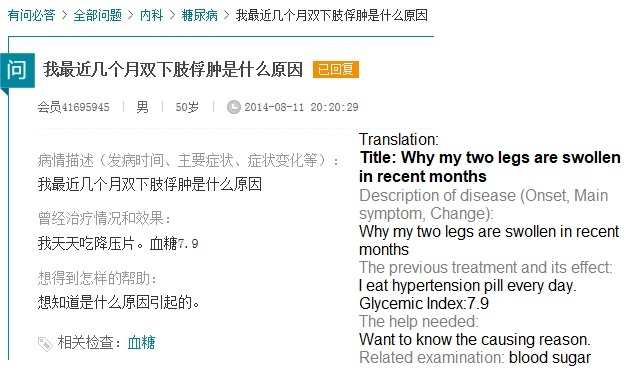
\includegraphics[width=0.9\columnwidth]{Fig2.jpg}
%	\resizebox{0.3\hsize}{!}{\includegraphics*{xywyExample.jpg}}
	\caption{Question posted on Xunyiwenyao website}
%	\definecolor{defGrey}{RGB}{128,138,135}
%	 Translation:\\
%		\textbf{Title: Why my two legs are swollen in recent months} \\
%		\textcolor{defGrey}{Description of disease (Onset, Main symptom, Change):}\\
%		Why my two legs are swollen in recent months\\
%		\textcolor{defGrey}{The previous treatment and its effect:}\\
%		I eat hypertension pill every day. Glycemic Index:7.9\\
%		\textcolor{defGrey}{The help needed:}\\
%		Want to know the causing reason.\\
%		\textcolor{defGrey}{Related examination:} blood sugar
	%	\\

	\label{fig:2}	
\end{figure}

\subsubsection{Chinese social media}
\label{subsubsec:2.2.1} 
Xunyiwenyao was established in 2004. By 2014, it has over 80,000,000 registered accounts, 
over 20,000,000 daily independent, and is ranked first in the medical and health service 
industry. The forum contains 14 categories and 64,050 discussion threads on average, 
every day. Each discussion thread starts with a patient’s question, which is followed by 
responses from multiple doctors or other patients (see Fig.~\ref{fig:2}).

Haodaifu was launched in 2006. Its physician-patient interactive forum is 
the largest in China, with over 501,000 registered healthcare professionals. 
It contains 29 categories and 18,632,602 discussion threads until now. 
The format of the discussion is similar to Xunyiwenyao.

\subsubsection{Extraction of evidences}
\label{subsubsec:2.2.3} 
First, we preprocess all the user posts from three websites. If one post contains a drug name of interest, this post is considered as an ``effective'' target. All sentences in ``effective'' posts are segmented by ICTCLAS \citep{zhang2003hhmm}, a Chinese word segmentation tool.

With the ADR lexicon, we can detect candidate ADR terms from the effective posts. However, when a drug name $X$ is mentioned in a post, the user may not actually have taken that drug. Similarly, when an ADR term is mentioned, the user may not actually have the symptom, or the symptom may not be the result of taking $X$. Therefore, given a pair of a drug name and an ADR, we need to determine whether the ADR is truly the consequence of taking the drug, given the context of the pair in the post. Because of that a drug-ADR pair that is too far away from each other in the text is not reliable, the context is defined as one or more consecutive sentences where the distance between drug and ADR is less than 55 Chinese words (including punctuations but excluding spaces). We ensure that each context contains one drug-ADR pair.

We define a context as a positive evidence if the candidate ADR in the context is a real ADR, while the other cases belong to the negative sentence. The following are two contexts showing a positive evidence and a negative evidence:

\begin{itemize}
	\item 服用\uline{易瑞沙}后\uline{头痛},眼睛复视,模糊 (After taking \uline{Iressa}, had a \uline{headache}, eye diplopia and blurred vision)
	\item 吃的是\uline{奥美拉唑},克拉霉素,阿莫西林,吗丁啉等药,\uline{咳嗽}有所减少 (After taking \uline{Omeprazole}, Clarithromycin, Amoxicillin, Domperidone and other drugs, \uline{cough} lessened) 
\end{itemize}

\subsubsection{Data set}
\label{subsubsec:2.2.4} 

\begin{table}
\centering
	% table caption is above the table
	\caption{Category of drugs studied}
	\label{tab:2}       % Give a unique label
	% For LaTeX tables use
	\begin{tabular}{llll}
%	\begin{tabular}{p{2cm}p{2cm}p{2cm}p{2cm}}
		%	\begin{tabular}{0.4\textwidth}{llll}
		\hline\noalign{\smallskip}
		Category & Number of drugs & Diseases & Number of drugs \\
		\noalign{\smallskip}\hline
		Hypertension & 29 & Hyperacidity & 2 \\
		Diabetes & 18 & Lung cancer & 1 \\
		Asthma & 15 & Rhinitis & 1 \\
		Statins & 9 & Schizophrenia & 1 \\
		Breast cancer & 1 & Acute coronary syndrome & 1 \\
		Anesthesia & 1 \\
		\noalign{\smallskip}\hline
	\end{tabular}
\end{table}


We have crawled user messages posted between January 2011 to April 2015 on Haodaifu and Xunyiwenyao. These messages mentioned 79 drugs, which treat 11 types of diseases. Table~\ref{tab:2} summarizes the diseases and the number of corresponding drugs. In total, 456,753 posts were crawled.

After preprocessing these posts, we obtain 302,180 sentences where a drug-ADR pair is revealed. We first manually label 1200 sentences which contains 600 positive evidences and 600 negative evidences. Then we divide them into training set, tuning set and test set. Finally, we get a training set with 300 positive evidences and 300 negative evidences, a tuning set with 200 positive evidences and 200 negative evidences and a test set with 100 positive evidences and 100 negative evidences.

\subsection{Evidence Classifier}
\label{subsec:2.3}
Given a drug name and a medical condition, identified by the extended lexicon, as well as their context in the original text, the problem of evidence classification is to determine whether the medical condition is actually an ADR resulting from the drug. Next we present a method to train such an evidence classifier. In particular, we show how to produce large amount of training data by automatic labeling.

\subsubsection{Building the training set}
\label{subsubsec:2.3.1} 
A supervised classifier requires labeled training data. However, manual labeling on user discussion posts can’t scale up because of the large amount of informal use of language and colloquial terms. Fortunately, information in the package insert of the drugs, e.g., the indications and the known side effects of the drug, can be used to automatically generate labeled data. 

Our first and simple idea is to regard a pair of drug and medical condition as true if the medical condition is listed as a side effect in the package insert of the drug. Conversely, we regard the pair as false if the medical condition is listed as an indication of the drug. All other pairs are discarded from labeled data set. However, this approach is not perfect. For example, “头晕(dizzyness)” is a known ADR for Betaloc, but sometimes in the real discussion it serves as an indication:

\begin{itemize}
	\item 突然感到\uline{头晕心慌},坐卧不安,去医院检查血压160.100 心电图心动过速160次,开了\uline{倍他乐克}(Suddenly I felt \uline{dizzy}, flustered, and restless, my blood pressure was at 160/100; tachycardia electrocardiogram was at 160 times. Consequently I was given \uline{Betaloc})
\end{itemize}

Similarly, “房颤(atrial fibrillation)” is an indication for Betaloc, but sometimes it is reported as if it’s a side effect:

\begin{itemize}
	\item 后根据医嘱,可达龙减至1/4片每天,加服\uline{倍他乐克}缓释片一片。一段时间后出现\uline{房颤}(According to the doctor’s advice, Cordarone was reduced to 1/4 tablets per day, plus one tablet of \uline{Betaloc}(slow release). \uline{Atrial fibrillation} occurred after a period of time)
\end{itemize}

Because the actual situation arising from patients’ experience may be more complicated than specified on the inserts, we adopt a semi-supervised approach instead. We first use the 
600 manually labeled data to train a simple SVM classifier and use it to predict for all 
the sentences in the corpus. The features used are discussed in 
Section \ref{subsubsec:2.3.2}. If the classifier predicts a sentence to be positive, 
and the medical condition is a known ADR for the drug according to the insert, 
we add this sentence into the new positive training set. If a sentence is predicted to be negative, and the condition in that sentence is a known indication of the drug, then we add this sentence into the negative training set. We exclude those sentences for which the 
prediction of classifier and content of the package insert are different. 
The new training set also contains our original 600 manual labeling data.

With little manual effort, we have now obtained a much larger set 
of positive and negative training data (called semi-supervised data) --- 
12,238 training instances in total. By manual validation, the accuracy of such 
automatic labeling is 82\%.

\subsubsection{Features extraction}
\label{subsubsec:2.3.2}
Our main evidence classifier extracts the following features (see Table\ref{tab:2.1}), after parsing the evidence sentences into dependency trees:

\begin{table}
	\centering
	\caption{Features that we extracted}
	\label{tab:2.1}       % Give a unique label
	% For LaTeX tables use
	%	\begin{tabular}{lllllll}
	\begin{tabular}{m{1.2cm}m{5cm}m{4cm}}
		\hline\noalign{\smallskip}
		Notation & Description & Examples \\
		\noalign{\smallskip}\hline\noalign{\smallskip}
		Feature 1 & Verbs before the drugs & “服用(take)” in “服用倍他乐克(take \textit{Betaloc})” \\
		Feature 2 & Verbs before the conditions & “感到(feel)” in “感到头晕(feel dizzy) \\
		Feature 3 & Verbs after the conditions & “好转(improved)” in “头疼好转(headache improved)” \\
		Feature 4 & Preposition, conjunction and noun of locality & “因为(because of)” in “因为头疼(because of headaches)” and “后(after)” in “服用倍他乐克后(after taking \textit{Betaloc})” \\
		Feature 5 & Punctuations that surround drugs and conditions & “,” and “。” in “吃完后,感到头疼。(feel headache after eating)” \\
		Feature 6 & The number of other drugs and other conditions between the drug and condition of interest & Both numbers are equaling to 1 in the sentence “服用信必可和舒利迭之后,感到头痛,身上有些地方还有荨麻疹(After taking \textit{Symbicort} and \textit{Seretide}, feel headache, there also appears urticaria in some places) if the drug and condition of interest is “信必可(Symbicort)” and “荨麻疹(urticaria)” \\
		Feature 7 & A boolean value that indicates whether condition appears in front of the drug or not & "true" in "因为哮喘,医生开了信必可(Because of asthma, the docter prescribed \textit{Symbicort})" and "false" for the sentence “用信必可来治疗哮喘(use \textit{Symbicort} to treat asthma)”\\
		\noalign{\smallskip}\hline
	\end{tabular}
\end{table}

\begin{comment}
\begin{enumerate}
	\item Verbs before the drugs, e.g. “服用(take)” in “服用倍他乐克(take \textit{Betaloc})”;
	\item Verbs before the conditions, e.g. “感到(feel)” in “感到头晕(feel dizzy)”;
	\item Verbs after the conditions, e.g. “好转(improved)” in “头疼好转(headache improved)”;
	\item Preposition, conjunction and noun of locality, e.g. “因为(because of)” in “因为头疼(because of headaches)” and “后(after)” in “服用倍他乐克后(after taking \textit{Betaloc})”;
	\item Punctuations that surround drugs and conditions;
	\item The number of other drugs and other conditions between the drug and condition of interest;
	\item A boolean value that indicates whether condition appears in front of the drug or not.
\end{enumerate}
\end{comment}
%The verbs are hard to extract without parsing the sentences. They often occur along with modifiers in the Chinese language. For example, “头疼好转(headaches improved)” would often be expressed as “头疼稍微好转(headaches improved a little bit)”, and with the dependency tree we can extract “好转(improved)” from it easily. 
The set of features described in Table\ref{tab:2.1} are used in both the initial and the final classifier. However, with more training data, the final classifier can better distinguish unseen tokens.
It’s worth noting that all these seven features are independent of the name of the drug 
and the ADR.

\subsubsection{Automatic labeling by bootstrapping}
\label{subsubsec:2.3.3}
We choose SVM as our primary classifier, because our feature vectors are high-dimensional (many different words). The overall process of our method is indicated in Algorithm.\ref{algo:bootstrap}.

\begin{algorithm}
	\caption{Automatic labeling by bootstrapping}
	\label{algo:bootstrap}
	\begin{algorithmic}[1]
		\State{Manually label small amount of seed data \textit{S}}
		\State{Train an initial SVM classifier M from \textit{S}}
		\State{Calculate F1-score of this SVM classifier based on the test data set}
		\Repeat
		%\While {F1-score not converge}
			\State{//Use \textit{M} to classify all the sentences and enlarge our training set with the help of packet inserts}
			\For {each sentence in corpus}
				\If {\textit{M} predicts this sentence to be positive \&\& the medication condition is a known ADR for the drug according to the packet insert}
					\State{Add this sentence to the positive training set}
				\ElsIf {M predicts this sentence to be negative \&\& the medication condition is a known indication of the drug according to the packet insert}
					\State{Add this sentence to the negative training set}
					\Else {\space keep this sentence in the corpus}
				\EndIf
			\EndFor
			\State{//update the SVM classifier}
			\State{Use the new training set to train a new SVM classifier and update \textit{M}}
			\State{Calculate F1-score of the updated classifier \textit{M} based on the test data set}
		%\EndWhile
		\Until {F1-score converge}
	\end{algorithmic}
\end{algorithm}


The above algorithm uses the package inserts and the initial classifier $M’$ to generate more training data. One interesting thought is to use that newly obtained classifier $M$ to label even more training data, and thus build a newer classifier. This process can go on iteratively until no more new training data is obtained. We will show the results of this in Section 3. The training data obtained at the final iteration is called semi-supervised data and will be used to train our SVM classifier and the other baseline classifiers (see Section~\ref{subsec:2.4}).

\subsection{Baseline classifier techniques}
\label{subsec:2.4}
\subsubsection{Pattern-based method}
\label{subsubsec:2.4.1}
Beside the above semi-supervised learning method, we have also tried a 
intuitive pattern-based classifier as a baseline. We extract preposition, 
conjunction and noun of locality from sentences as patterns from training data generated 
by package inserts. Each pattern has a weight, which is its frequency of occurrence; 
a negative pattern extracted from negative examples will have a negative weight. 
For example, below are two patterns we extracted and their weight:

\begin{itemize}
	\item drug ... 后 ... adr ... \quad 20
	\item adr ... 后 ... drug ... \quad -3
\end{itemize}

For a new sentence that can be matched to several patterns, the score is the sum of these patterns. Then a classifier is built based on the score: if the score is greater than 0, it’s positive; otherwise negative.

\subsubsection{HMM-based classifier}
\label{subsubsec:2.4.2}
We train a HMM classifier \citep{sampathkumar2014mining}. Particularly, comparing to original HMM paper where the sentences to be classified may not contain a drug-ADR pair, our task is more challenging because we firstly ensure a drug-ADR pair in all sentences and then make the classification.
We train two HMM classifiers in all. One classifier is only trained with 600 manually-labeled data and another classifier is trained with the semi-supervised data by using the package insert.

\subsubsection{CRF-based classifier}
\label{subsubsec:2.4.3}
We train a CRF-based classifier \citep{nikfarjam2015pharmacovigilance}. We also use two kind of data to train the two CRF-based classifiers: one with 600 manually-labeled data and another with semi-supervised data.
\\

Both the HMM and CRF classifiers were slightly modified to adapt to the Chinese input. For example we use ICTCLAS to segment and POS to tag the input sentences. 

\subsection{Ranking}
\label{subsec:2.5}
For each drug, there are many candidate ADRs. We are interested in those of high confidence. 
One way of ranking the ADRs of a drug is by the number of its appearances in positive 
evidence posts. This doesn’t work well because, most discussions about a drug involves the 
indications of the drug. For example, discussion about \textit{Betaloc} would naturally 
include a lot of occurrences of the term ``hypertension'' and the absolute number of such 
mentions is very large. Although our classifier can give a high accuracy, 
a number of sentences which contains ``hypertension'' as ADR are incorrectly predicted to 
be positive. Consequently, ``hypertension'' would be ranked highly as an ADR of 
\textit{Betaloc}. To solve this problem, we rank the ADRs according to the frequency of 
the positive evidences minus that of the negative evidences. This approach effectively 
lowers the rankings of the indications of a drug, but promotes real ADRs.
